\documentclass[a4paper, 11pt]{article}
\usepackage[left=2cm, top=3cm, text={17cm, 24cm}]{geometry}
\usepackage[utf8]{inputenc}
\usepackage[czech]{babel}
\usepackage{graphicx}
\usepackage{verbatim}
\usepackage{enumitem}
\usepackage{times}
\usepackage[unicode]{hyperref}

\begin{document}

    \catcode`\-=12

    \begin{titlepage}
        \begin{center}
            {\Huge\textsc{
                        Fakulta informačných technológií \\
                        Vysoke učení technické v~Brně \\
            }}
            \vspace{\stretch{0.382}}
            {\Large
                        \Huge {Projektová dokumentácia} \\
                        \LARGE {\textbf {Implementácia prekladača imperatívneho jazyka IFJ19}} \\
                        \vspace{\stretch{0.018}}
                        \large{Tím 033, varianta I}}
                        \vspace{\stretch{0.600}}
        \end{center}
    
        \hfill            
        \begin{minipage}[r]{0.49 \textwidth}
                \Large
                \begin{tabular}{l l l}
                    \textbf{Maroš Geffert} & \textless \textbf{xgeffe00}\textgreater & \quad 25\, \% \\
                    Patrik Tomov & \textless xtomov02\textgreater  & \quad 25\, \% \\
                    Martin Valach & \textless xvalac12\textgreater  & \quad 25\, \% \\
                    Andrej Pavlovič & \textless xpavlo14\textgreater  & \quad 25\, \% \\
                \end{tabular}
        \end{minipage}   
        
        \begin{minipage}[r]{0.4 \textwidth}
                {\Large \today}
        \end{minipage}    
        
    \end{titlepage}    
    
    
    %%%%%%%%%%%%%%%%%%%%%%%%%%%%%%%%%%%%%%%%%%%%%%%%%%%%%%%%%%%%%%%%
    \pagenumbering{arabic}
    \setcounter{page}{1}
    \tableofcontents
    \clearpage
    
    %%%%%%%%%%%%%%%%%%%%%%%%%%%%%%%%%%%%%%%%%%%%%%%%%%%%%%%%%%%%%%%
    \pagenumbering{arabic}
    \setcounter{page}{1}
    
    \section{Úvod}
    Cieľom nášho projektu bolo vytvoriť prekladač v~jazyku C, kotrý načíta zdrojový súbor zapísaný v~zdrojovom jazyku IFJ19, ktorý reprezentuje podmnožinu jazyka Python 3, a preloží ho do~cieľového jazyka IFJcode19. V prípade chyby vracia odpovedajúci chybový kód.
    
    \section{Implementácia}
    
    \begin{figure}[h]
		\centering
		\scalebox{0.45}{
			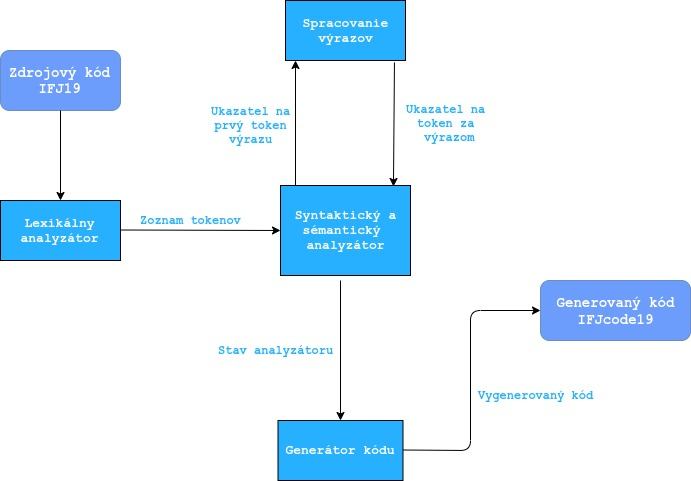
\includegraphics{inc/IFJ19.jpg}
		}
	\end{figure}
    
    \subsection{Lexikálny analyzátor}

    Pri programovaní prekladača, sme začínali s~tvorbou lexikálneho analyzátoru. Základnou funkciou tejto časti je funkcia \texttt{get\_token}, vďaka ktorej je možne načítávať lexémy\footnotemark zo~zdrojového súboru a~prevádzajú sa do~podoby takzvanej token. Token je štruktúra ktorá obsahuje (atribúty, typy, v~prípade identifikátoru si uchováva aj jednotlivý string atď.). Typy tokenov môžu byť klúčove slová, identifikator, rôzne operátory, EOL, EOF a~všetko čo jazyk IFJ19 podporuje. Jednotlivé atribúty sa k~tokenom priradzujú podľa situácie (napr. pre identifikátor alebo čísla (float, integer).
    
    Lexikálny analyzátor funguje ako deterministický konečný automat. Tento konečný automat sme implementovali ako opakujúci sa switch, kde každý case odpovedá nejakému stavu z~automatu. Ak sa načítaný lexem nezhoduje so~žiadným odpovedajúcim stavom určeným jazykom IFJ19 tak vraciame chybu 1. Lexikálna analýza končí načítaním posledného znaku zo~zdrojového súboru, ktorým je \texttt{EOF} (Prípadne skončí v~chybovom stave pri~internej chybe). 

        
    \footnotetext{Lexéma je základná jednotka lexikálnej (čiže slovnej) zásoby jazyka, t.j. základná jazyková jednotka, ktorá je nositeľom vecného významu.}    
    \pagebreak    
        
    \subsection{Syntaktická a sémantická analýza}
    
    Najpodstatnejšou časťou prekladača je syntaktická a sémantická analýza tzv. Parser. Parser je založený na rekurzívnom zostupe z~hora dolu. Jeho úlohou je kontrola, či reťazec tokenov reprezentuje syntaktický správne napísaný program v jazyku IFJ19, pričom zároveň prebieha aj sémantika programu, kde sa kontroluje či je daná premenná definovaná, správny počet argmentov pri~volaní funkcie, kompatibilita dátových typov a pod.

    V~rekurzívnom zostupe si žiadame postupne tokeny od scanneru pomocou funkcie \texttt{get\_token} a na základe LL pravidiel postupujeme. Každé pravidlo má svoju vlastnú funkciu. Každá takáto funkcia má parameter ukazateľ na~\texttt{Parser\_data}, čo je štruktúra, ktorá obsahuje potrebné premenné na vykonanie syntaktickej a sémantickej analýzy. V~prípade, že dojde k~chybe, program končí s návratovou hodnotou chyby, ktorá sa vypíše. Táto časť taktiež úzko súvisí s~tabuľkou symbolov, ktorá slúži na~ukladanie názvov premenných a funkcií(sémantika).

    Spracovanie výrazov sa taktiež vykonáva v~parsri. Spracovanie spočíva v~skontrolovaní priorít výrazov (pomocou syntaktickej analýzy PSA popísanej nižšie) a skontrolovaní premenných, u~ktorých sme schopný skontrolovať dátové typy pri preklade, resp. sme ich schopný pretypovať (jediné povolené pretypovanie je z~integeru na float) V prípade zlej kombinácie dátových typov vraciame chybu 4. Výrazy, ktoré niesme schopný zkontrolovať za~prekladu (napr. premenné, ktoré môžu byť definované v~hlavnom tele; parametre funkcií; atď.) kontroluje generátor kódu.
        
    \subsection{Generovanie kódu}
    
    Generovanie výstupného kódu IFJcode19 na~štandardný výstup prebieha až po~úspešnom ukončení prekladača. Dovtedy sa kód ukladá na~jeho internú pamäť. Na~generovanie kódu sa využívajú prevažne makrá. Funkcie, kotré generujú kód sú samostatne oddelené v~\texttt{code\_generator.c}. Pri~štarte prekladača sa generuje hlavička ktorá obsahuje vstavané funkcie jazyka a preddefinované pomocné globálne premenné využívané pri~rôznych operáciách. Funkcie na~generovanie kódu sú rozdelené na~jednoduché operácie (priradenie, hlavičky a pätičky pre podmienené príkazy, atď.), ktoré sú volané syntaktickou analýzou podľa potreby. Priamo do~generovaného kódu väčšina funkcií hneď na~začiatku generuje aj jednoriadkový komentár ktorý stručne popisuje čo táto funkcia vykonáva.

    \subsection{Interpret}
    
    Interpret vytvára interpretáciu trojadresného kódu, generovaného syntaktickým analyzátorom. Trojadresný kód je uloženy v~instrukčnom liste, ktorý je implementovaný pomocou jednosmerného viazaného lineárneho zoznamu. Pre každú inštrukciu je tento kód reprezentovaný typom inštrukcie, adresou výsledku a~adresami prvého a~druhého operandu. Pri spracovávaní aritmeticko-relačných operácií robí interpret sémantickú kontrolu.
    
    \pagebreak
    \section{Algoritmy}
    \subsection{Dynamický string}
    
    Prvý algoritmus, ktorý sme použili je \texttt{Lexem\_string} pre operácie s~reťazmi rôznej dĺžky. Štruktura má v~sebe uložene ukazatel na~reťazec, dĺžku reťazca a~aj koľko pamäte je vyhradené pre~reťazec. Implementované operácie : inicializácia (Pri inicializácii sa vyhradí pamäť práve pre~určitý počet znakov a~ak je potrebné tak sa realokuje), uvoľnenie dát, pridanie znaku alebo stringu do reťazca atd.
    
    \subsection{Precedenčná tabuľka}
    
    Na~vyhodnocovanie priorít vykonávaných operácií pri~výrazoch sme implementovali precedenčnú syntaktickú analýzu (PSA). PSA vo~svojom algoritme využíva precedenčnú tabuľku, ktorú sme implementovali ako dvojrozmerné pole, v~ktorej sú zapísané všetky možné operácie ktoré môže nastať a sú v~nej zároveň porovnané. Pre porovnávanie využívame zásobník, na~ktorom je vždy terminal (operátor, ktorý bol spracovaný), ktorý porovnávame so~znakom, ktorý sme dostali zo~vstupu (pomocou funckie \texttt{get\_token} a následného spracovania pre~index tabuľky, pomocou funkcií \texttt{get\_symbol} a \texttt{get\_index)} a v~podľa výsledku porovania vykoná pravidlo PSA. PSA pokračuje pokým nie je celý výraz zkontrolovaný, prípadne pokým v~ňom nenájde chybu.
    
    
    
    \subsection{Tabuľka symbolov}
    
    Tabuľku symbolov sme implementovali ako tabuľku s rozptýlenými položkami(hash function). Keďže rozlišujeme, či je premenná globálna alebo lokálna tak rozlišujeme aj globálnu a lokálnu tabuľku. V tabuľke symbolov sa nachádzaju položky, ktoré reprezentuje štruktúra
    \texttt{Sym\_table\_item}, ktorá obsahuje: char* key(názov), ktorý slúži taktiež na pridelenie indexu v tabuľke na základe hashovacej funkcie. IData data je štruktúra, ktorá obsahuje informácie o položke. Medzi informácie ktoré obsahuje patrí či bola premenna definovaná, či je globálna alebo lokálna a štruktúru \texttt{Sym\_table\_item *next}, čo je ukazateľ na ďalší item.
    
    \section{Práca v tíme}
    
    Náš tím sa stretol po~zadaní projektu. Vedúcim tímu boli hneď aj rozdelené úlohy. Tím väčšinou medzi sebou komunikoval osobne alebo cez discord. 
    
    Najprv sme si stanovili štruktúru celého projektu. V~priebehu prvých šiestich týždňov sa toho veľmi neurobilo, implementoval sa lexikálny analyzátor, členovia študovali a~zbierali informácie ohĺadom svojej časti programu, ktorá im bola zadaná vedúcim tímu. V~priebehu ďalších týždňov sme implementovali celý program. Testovali sme jednotlivé časti osobitne, ale neskôr sme to už testovali spolu ako celok. K~zdieľaniu kódu sa používal repozitár git.
    
    \begin{tabbing}
    meno ~~~~~~~~~~~~~~~~~~~~\= login ~~~~~~~~~~~
    \= rozdelenie práce \kill
    \bfseries Meno \>
    \bfseries Login \>
    \bfseries Rozdelenie práce \\[2mm]
    Maroš Geffert \> xgeffe00 \> Lexikálna analýza, dokumentácia, testy, testovací skript \\
    Patrik Tomov \> xtomov02 \> Syntaktická analýza, testy\\
    Martin Valach \> xvalac12 \> Sémantická analýza \\
    Andrej Pavlovič \> xpavlo14 \> Generátor kódu
    \end{tabbing}

    \pagebreak
    \section{Záver}
    
    Projekt nás až tak nezarazil, vzhľadom nato, že sme sa naňho začínali pripravovať v~celku dosť skoro. Tím sme si zostavili veľmi rýchlo a~tým, že sme na~rovnakom internáte tak nebol problém s~akoukoľvek komunikáciou. Jednotlivé časti programu sme riešili z~väčšej časti individuálne.
    Správnosť projektu sme si overili automatickými testami a~pokusným odovzdaním, vďaka ktorému sme boli schopní projekt viac doladiť.
    
    Na tomto projekte sme si vyskúšali implementáciu niektorých zaujímavých dátových štruktúr, algoritmov, teóriu formálnych jazykov v~praxi a~spoluprácu v tíme.
    
    \clearpage
    
    \section{Digramy}
    \subsection{Deterministický konečný automat popisujúci lexikálnu analýzu}
    \begin{figure}[h]
		\centering
		\scalebox{0.5}{
			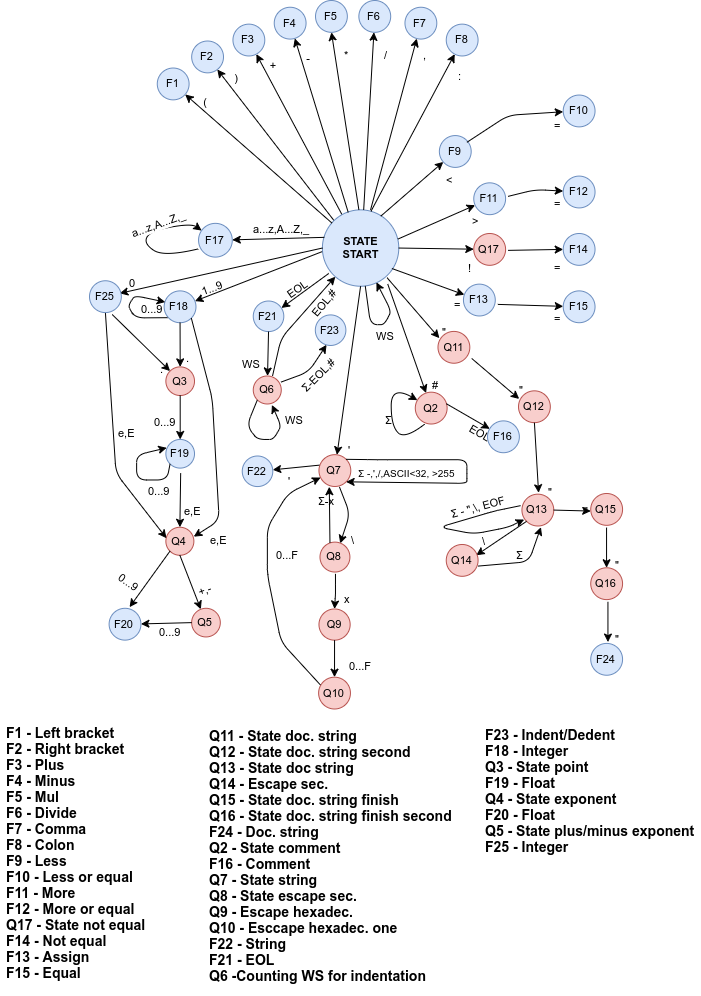
\includegraphics{inc/scanner.png}
		}
		\caption{Deterministický automat špecifikujúci lexikálny analyzátor}
	\end{figure}
	
	\pagebreak
	
	\subsection{Precedenčná tabulka}
    \begin{figure}[h]
		\centering
		\scalebox{0.5}{
			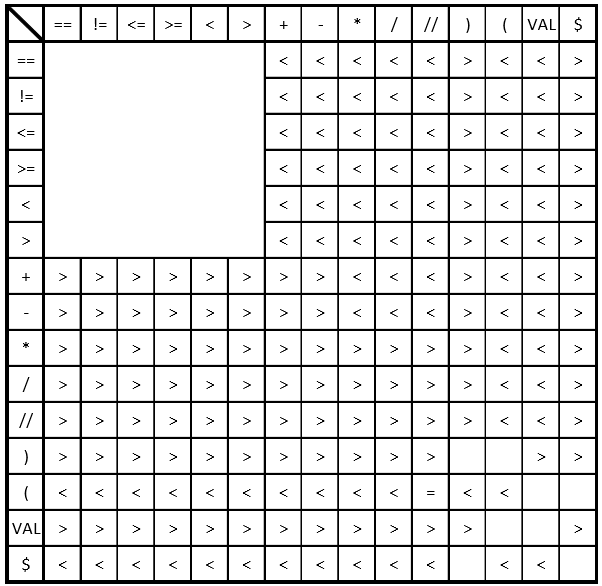
\includegraphics{inc/table.png}
		}
		\caption{Precedenčná tabuľka použitá pri analýze výrazov}
	\end{figure}

    \pagebreak
    
    \subsection{LL}
    \subsubsection{LL gramatika}
    \begin{figure}[h]
		\centering
		\scalebox{0.5}{
			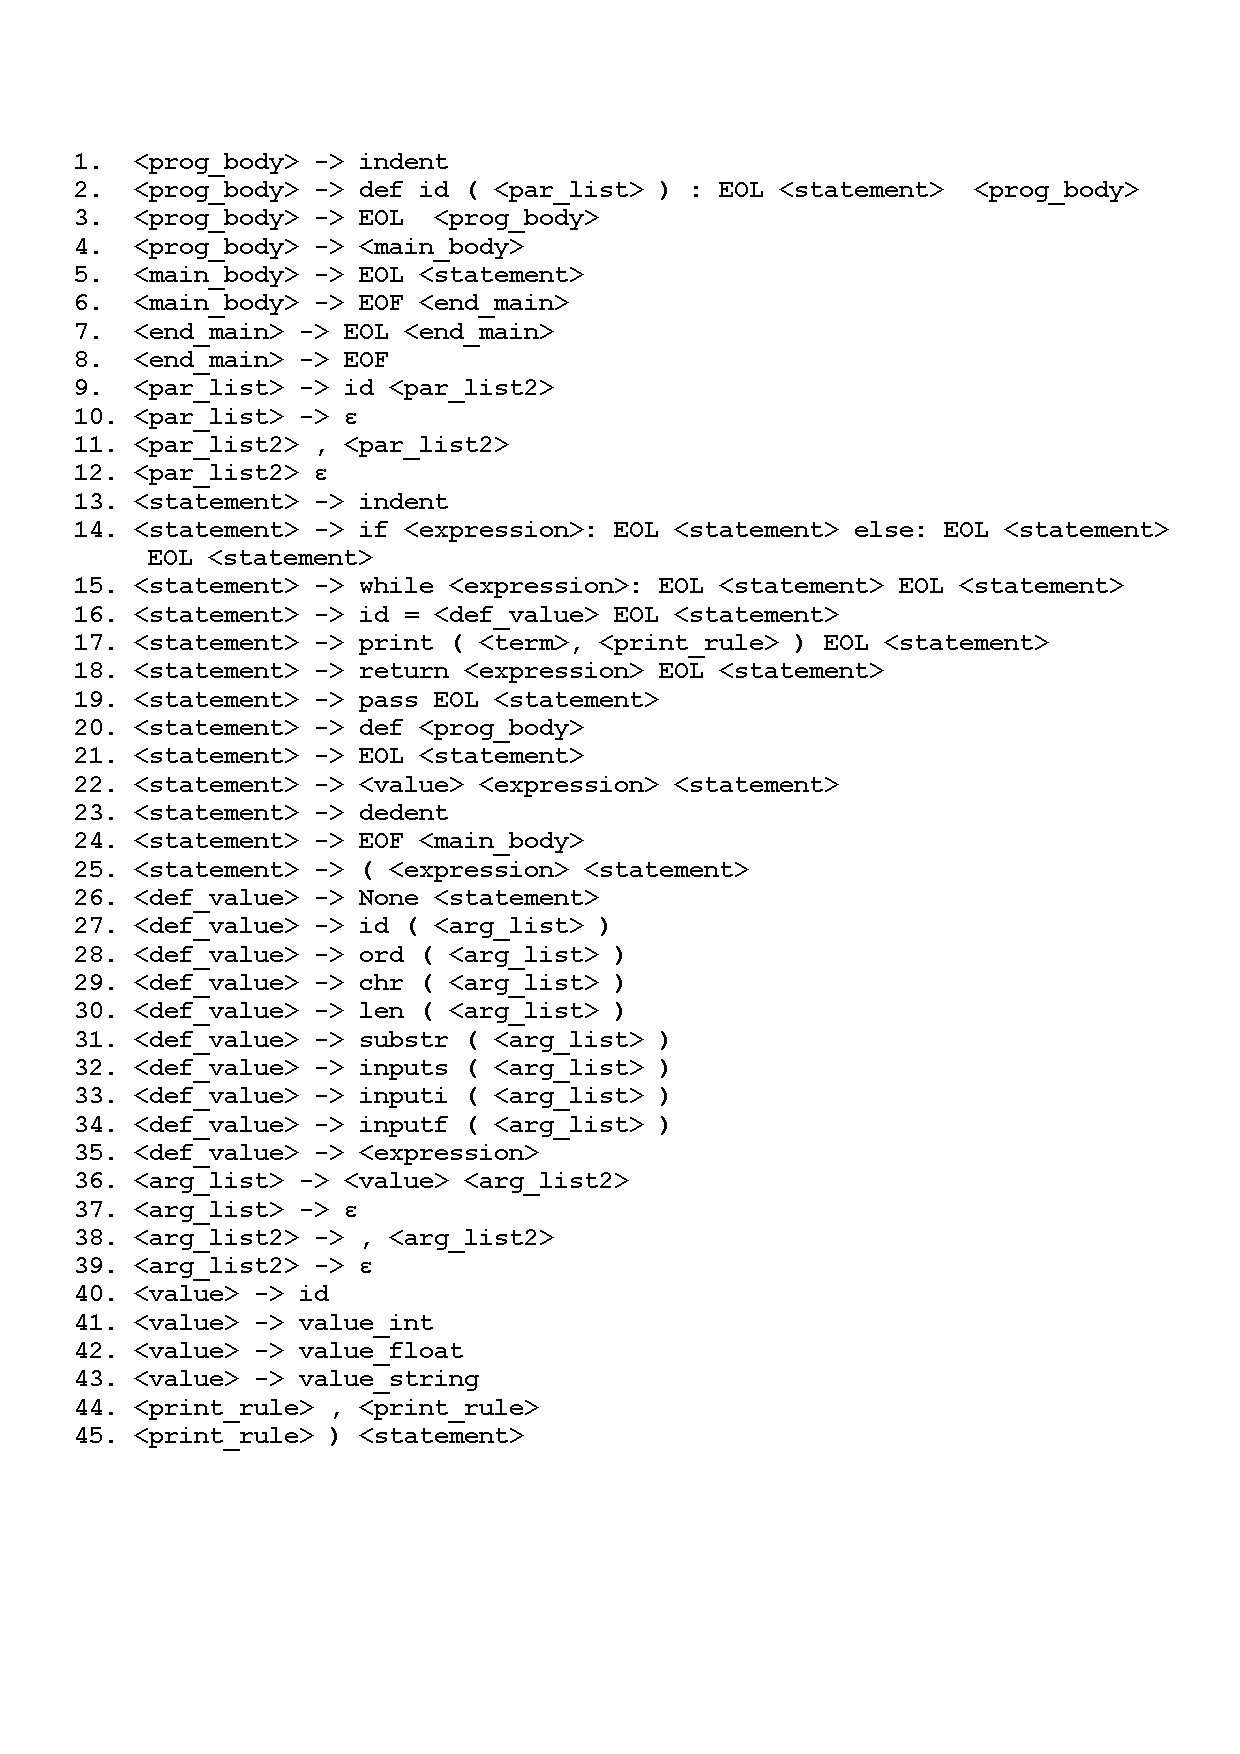
\includegraphics{inc/LL-gramatika.pdf}
		}
		\caption{Pravidlá LL gramatiky pre syntaktickú analýzu}
	\end{figure}
	\pagebreak
    \subsubsection{LL Tabuľka}
    \begin{figure}[h]
		\centering
		\scalebox{0.5}{
			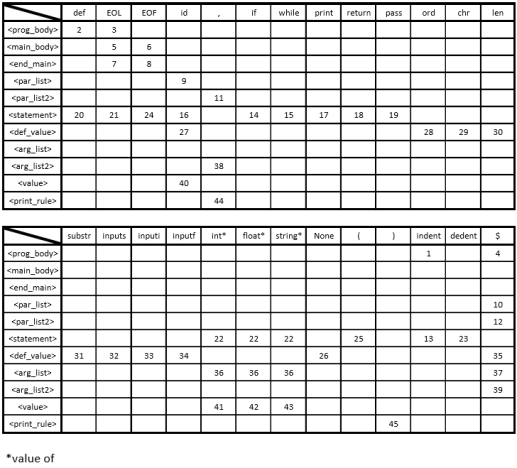
\includegraphics{inc/LL_tablee.png}
		}
	    \caption{LL tabuľka}
	\end{figure}

\end{document}
